\subsection{Red Laboral}

Esta captura se realizó en la red laboral de uno de los integrantes del grupo. Al ser una red con una gran cantidad de nodos y tráfico de paquetes, se optó por hacer las capturas al final de la jornada laboral donde el tráfico es menor. En otro momento los gráficos no resultaban claros para su análisis. La captura se realizó durante aproximadamente 10 minutos.
\\\\
Vemos a continuación el gráfico que muestra la topología de la red según el intercambio de paquetes ARP que hubo en la captura.

\begin{figure}[ht!]
  \centering
   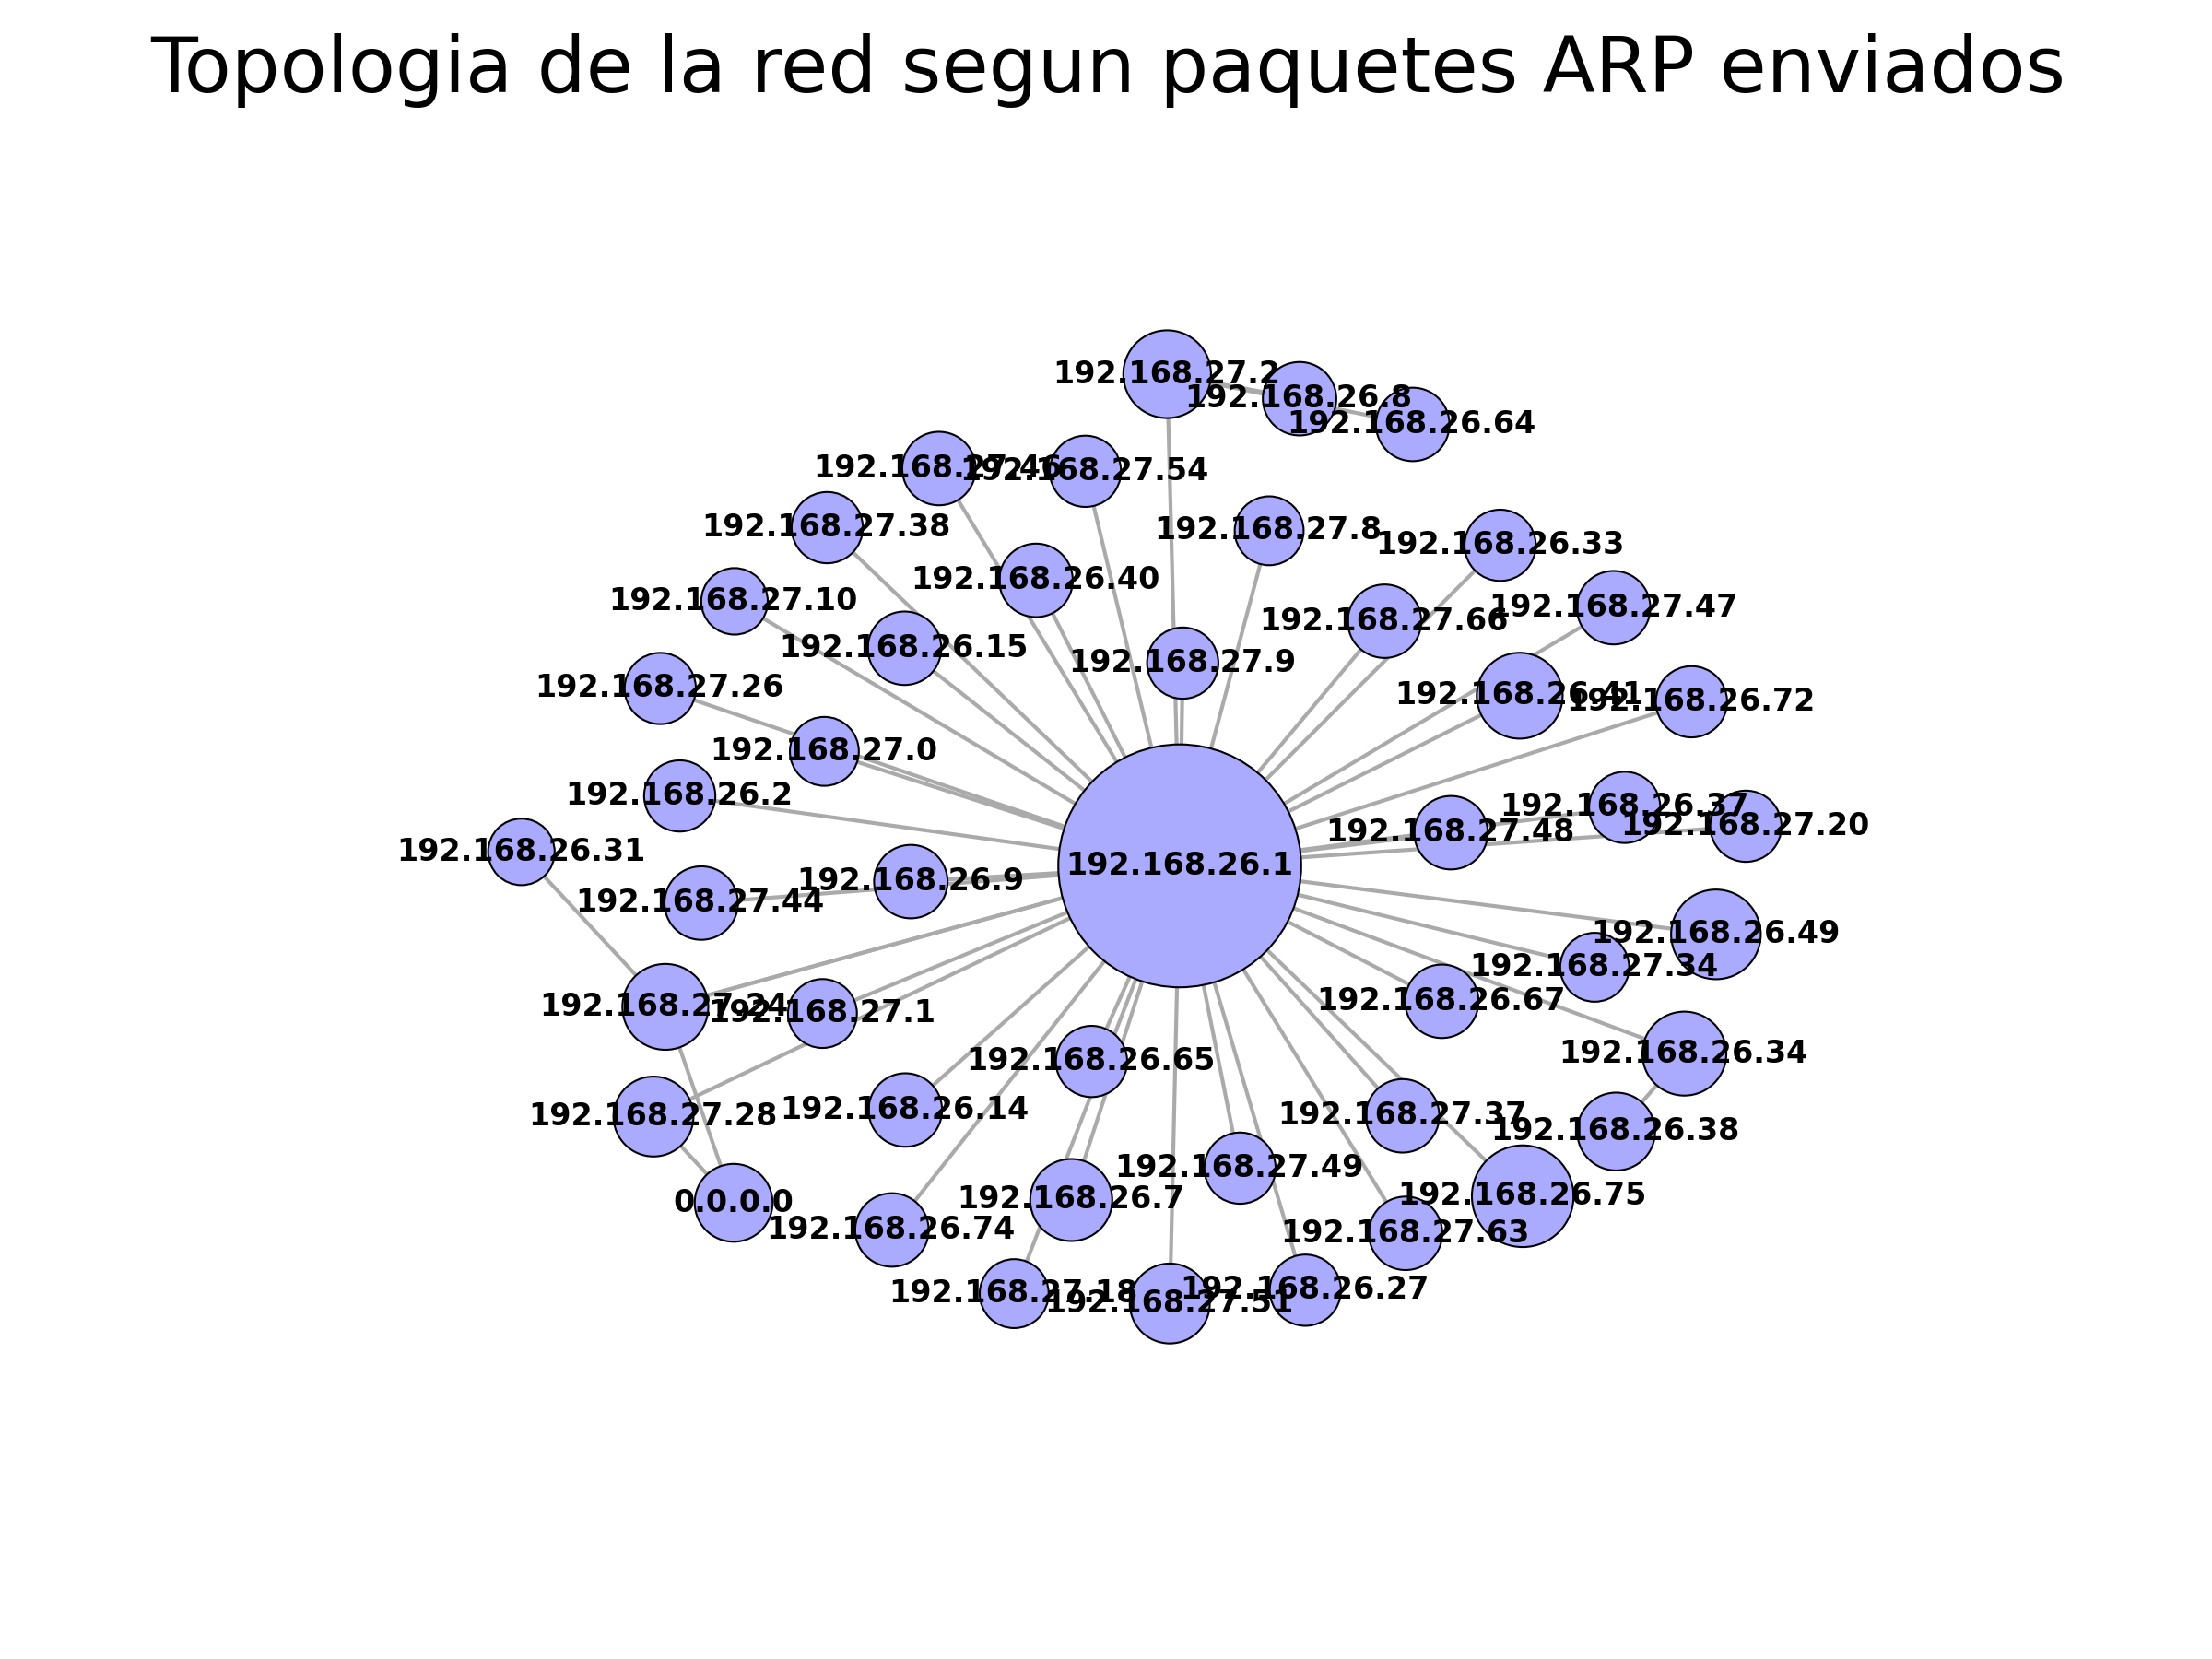
\includegraphics[width=0.7\textwidth]{graficos/laboral_network.png}
  \caption{}
  \label{fig:laboral_network}
\end{figure}

En el centro del gráfico y de mayor tamaño podemos observar el nodo que representa al router con dirección IP 192.168.26.1. Por destacarse frente a los demás nodos creemos que este podría ser el nodo distinguido.
\\\\
Vemos ahora el gráfico que muestra la cantidad de información de cada nodo con respecto a la entropía.

\begin{figure}[ht!]
  \centering
   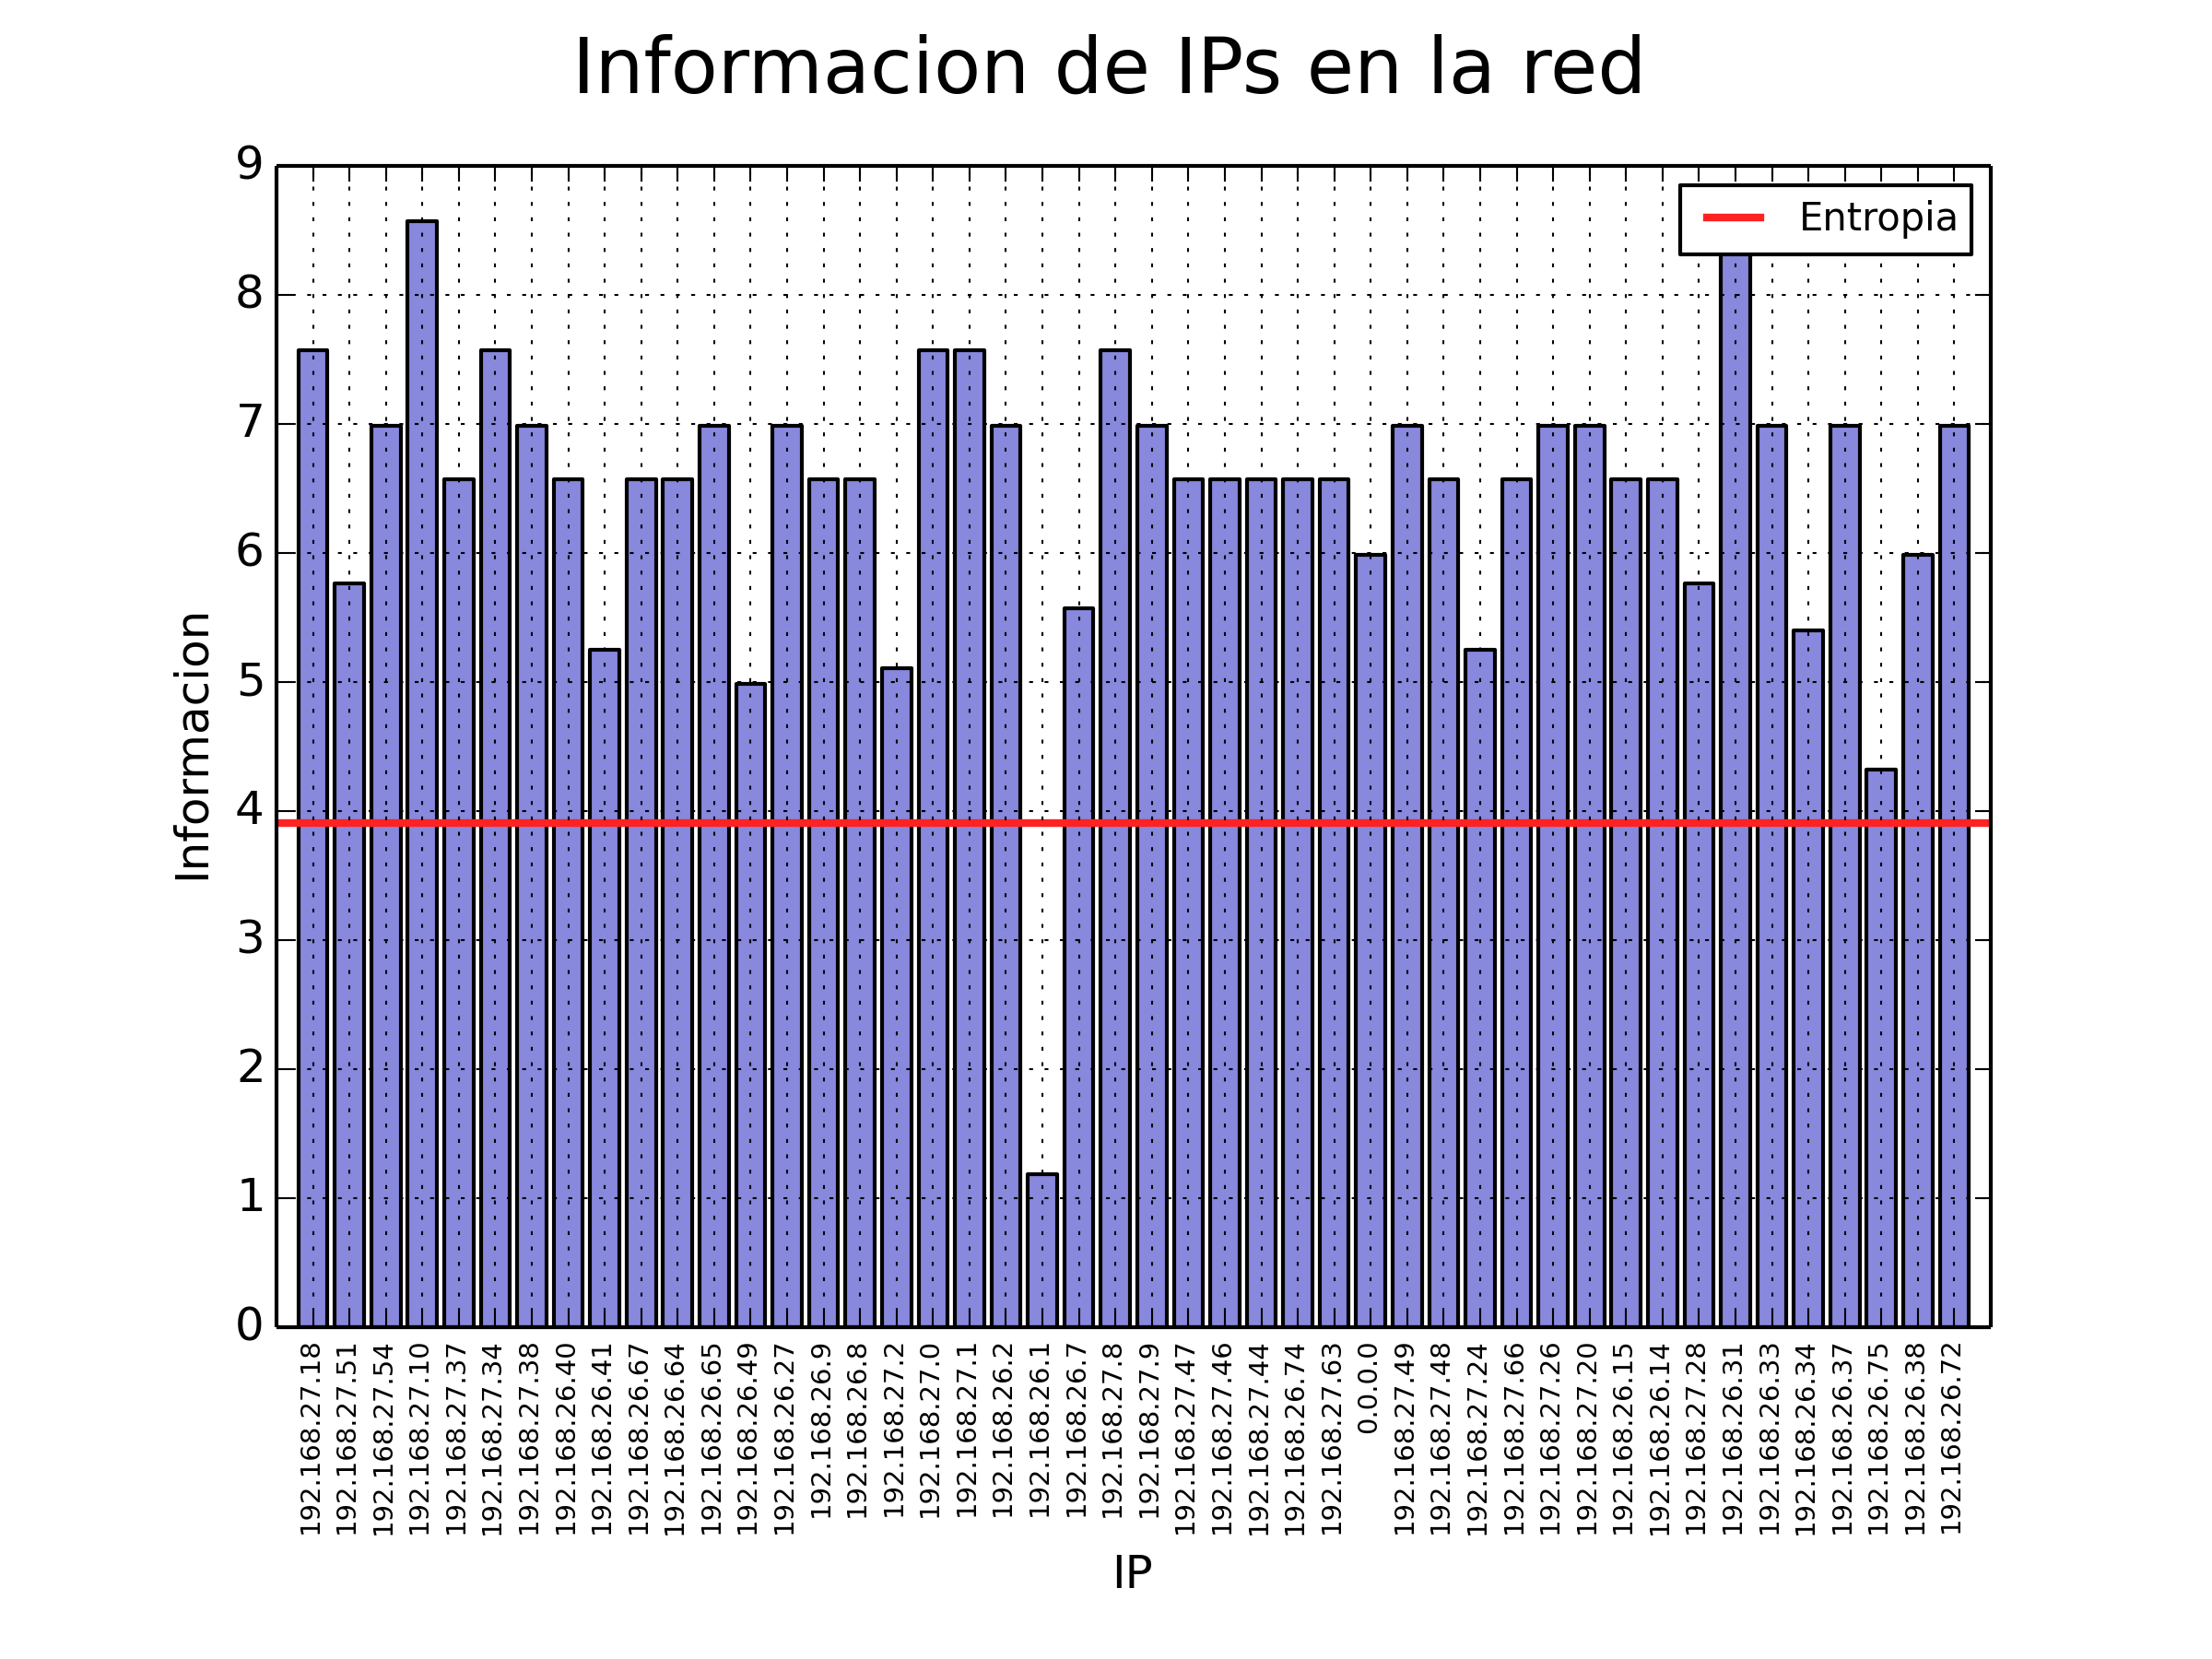
\includegraphics[width=0.7\textwidth]{graficos/laboral_information_bars_arp.png}
  \caption{}
  \label{fig:laboral_information_bars_arp}
\end{figure}

Como podemos comprobar en este gráfico, la información que presenta el nodo correspondiente al router se encuentra muy por debajo de la entropía de la fuente. Por lo tanto concluímos que este es un nodo distinguido. Por otro lado vemos a un par de nodos que aportan mucha información, o sea que presentan una baja probabilidad. Posiblemente estos dos nodos sean equipos que tuvieron poca actividad durante la captura de paquetes, y participaron en pocas búsquedas ARP.
\\\\
Veremos a continuación el gráfico que muestra la cantidad de información de cada protocolo en comparación con la entropía.

\begin{figure}[ht!]
  \centering
   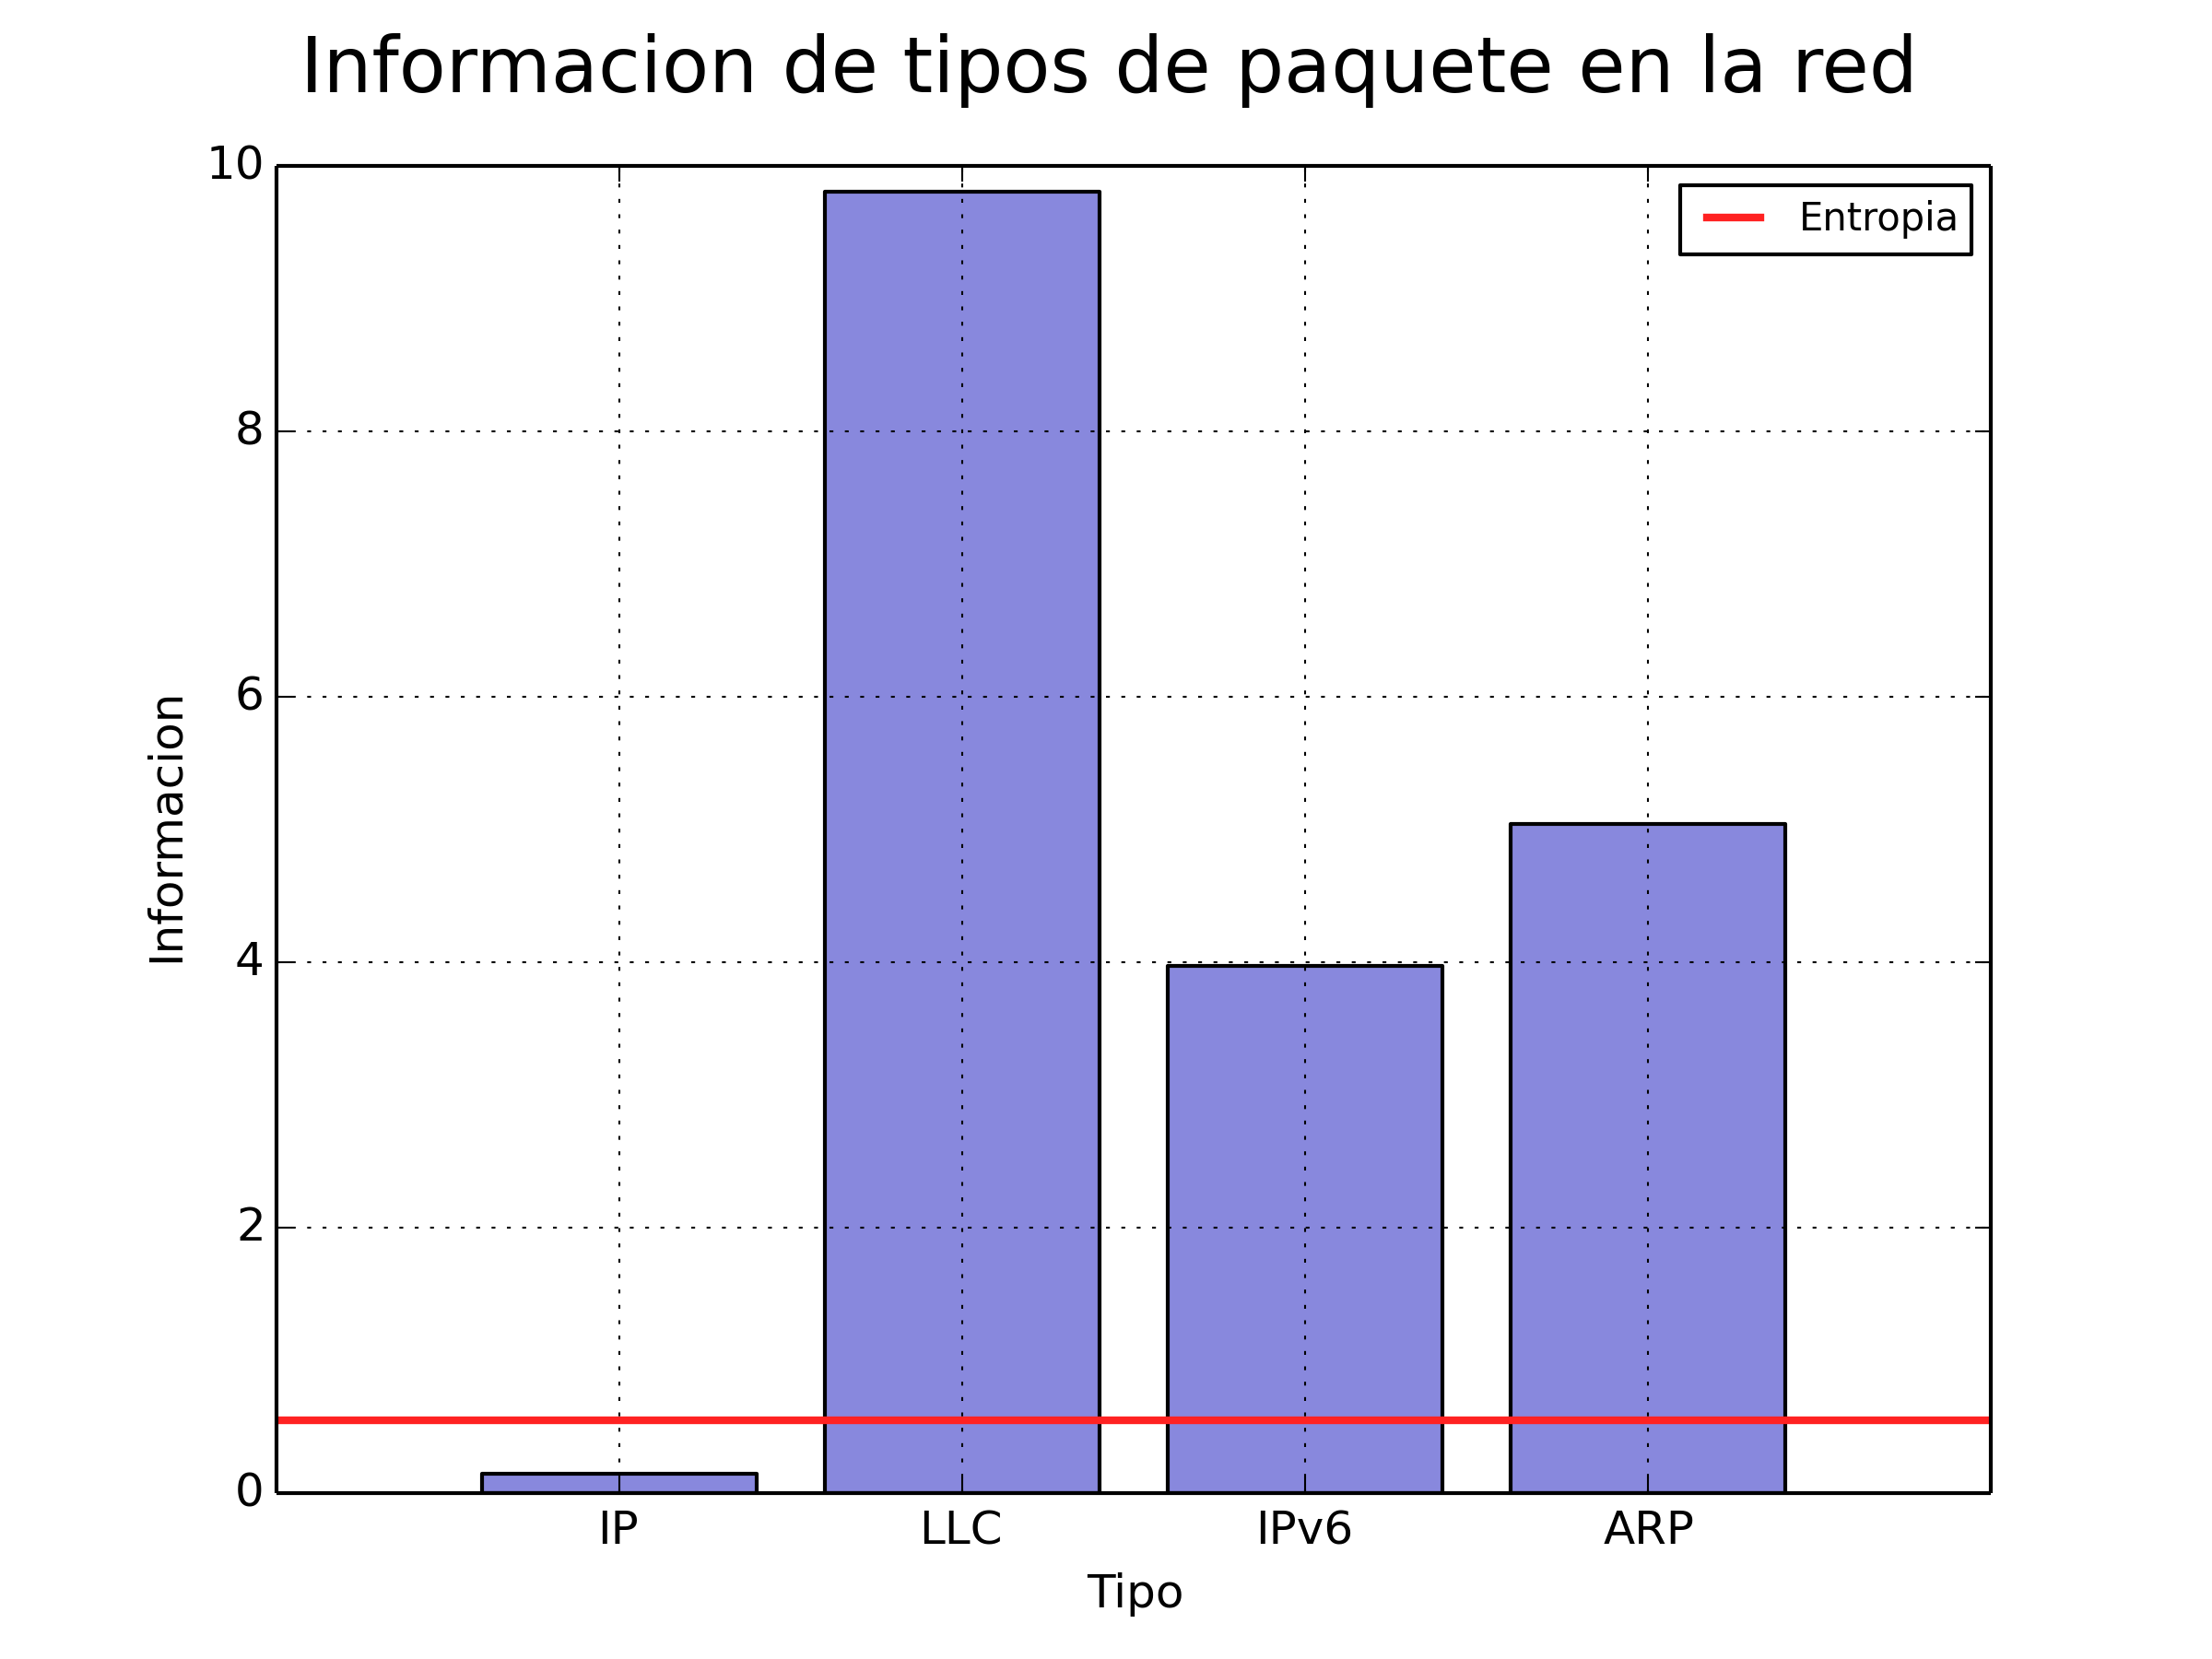
\includegraphics[width=0.7\textwidth]{graficos/laboral_information_bars_type.png}
  \caption{}
  \label{fig:laboral_information_bars_type}
\end{figure}

Se pueden observar dos símbolos distinguidos. El protocolo IPv4, cuya información se presenta por debajo de la entropía. Es el protocolo que presenta más frecuencia y por este motivo aporta muy poca información.
Y el protocolo LLC que con muy poca frecuencia nos da mucha información.
También podemos observar que la cantidad de paquetes ARP e IPv6, en comparación con la de IPv4, es baja.